%% ============================================================
%% DV-SLAM — Abstract + Section I (Introduction)
%% IEEE RA-L format
%% New framing: sparse dToF LIO (no confidence as contribution,
%% no camera-free claims, no Propositions 1-2 in contributions)
%% ============================================================

\begin{abstract}
Existing LiDAR-inertial odometry (LIO) systems assume dense point clouds
($>$10K points/scan) produced by mechanical spinning LiDARs.
Consumer direct time-of-flight (dToF) sensors, now embedded in hundreds
of millions of smartphones, deliver only 200--500 usable points per frame
after quality filtering — two orders of magnitude fewer.
No open LIO system has been designed for, or validated in, this sparse regime.
We present DV-SLAM, a tightly-coupled LiDAR-inertial-visual odometry system
built from the ground up for sparse mobile dToF hardware.
Three design choices make LIO viable below 500 points per frame:
(i)~a lightweight voxel-hash map (O(1) insert, LRU eviction, 500K-cell cap)
replacing the ikd-tree used by dense-cloud systems;
(ii)~stride-sampled ESKF updates (max 100 observations per frame) that reduce
LDLT cost by $125\times$ relative to processing full dense-LiDAR scans; and
(iii)~tight fusion of depth point-to-plane residuals and monocular visual
reprojection residuals in a single iterated ESKF update.
The entire pipeline — IMU propagation, visual feature tracking, and
point-to-plane ICP — executes on-device at 30\,Hz on an iPhone\,15\,Pro\,Max
(Apple A17 Pro SoC) with a single Eigen dependency and no external hardware.
We characterize the sparse regime empirically via a point-count sweep
(50--3{,}000 points/frame on ScanNet++ sequences), identifying the collapse
boundary below which stable LIO is no longer achievable.
Evaluated against FARO ground-truth on ScanNet++ (ICCV 2023),
DV-SLAM achieves competitive trajectory accuracy and substantially outperforms
naive ICP and IMU-dead-reckoning baselines, demonstrating that robust LIO
is achievable on a sensor class previously considered too sparse for odometry.
\end{abstract}

\begin{IEEEkeywords}
LiDAR-inertial odometry, direct time-of-flight, mobile 3D scanning,
sparse point cloud, error-state Kalman filter, on-device SLAM.
\end{IEEEkeywords}

%% ============================================================
\section{Introduction}
\label{sec:intro}
%% ============================================================

%% P1: Dense LIO has succeeded — but on rich hardware
\IEEEPARstart{S}{ystems} such as FAST-LIO2~\cite{xu2022fastlio2}
and DLIO~\cite{chen2023dlio} routinely achieve centimeter-level
trajectory estimation on mechanical scanning LiDARs
that produce 10{,}000--130{,}000 points per scan.
KISS-ICP~\cite{vizzo2023kiss} showed that even simple point-to-point
ICP with adaptive thresholding rivals more complex pipelines when the
point cloud is sufficiently dense.
These results have established LIO as a mature technology — but on
hardware that costs thousands of dollars per sensor and is
impractical to embed in a handheld smartphone.

%% P2: dToF is now ubiquitous but qualitatively different
\begin{figure*}[t]
    \centering
    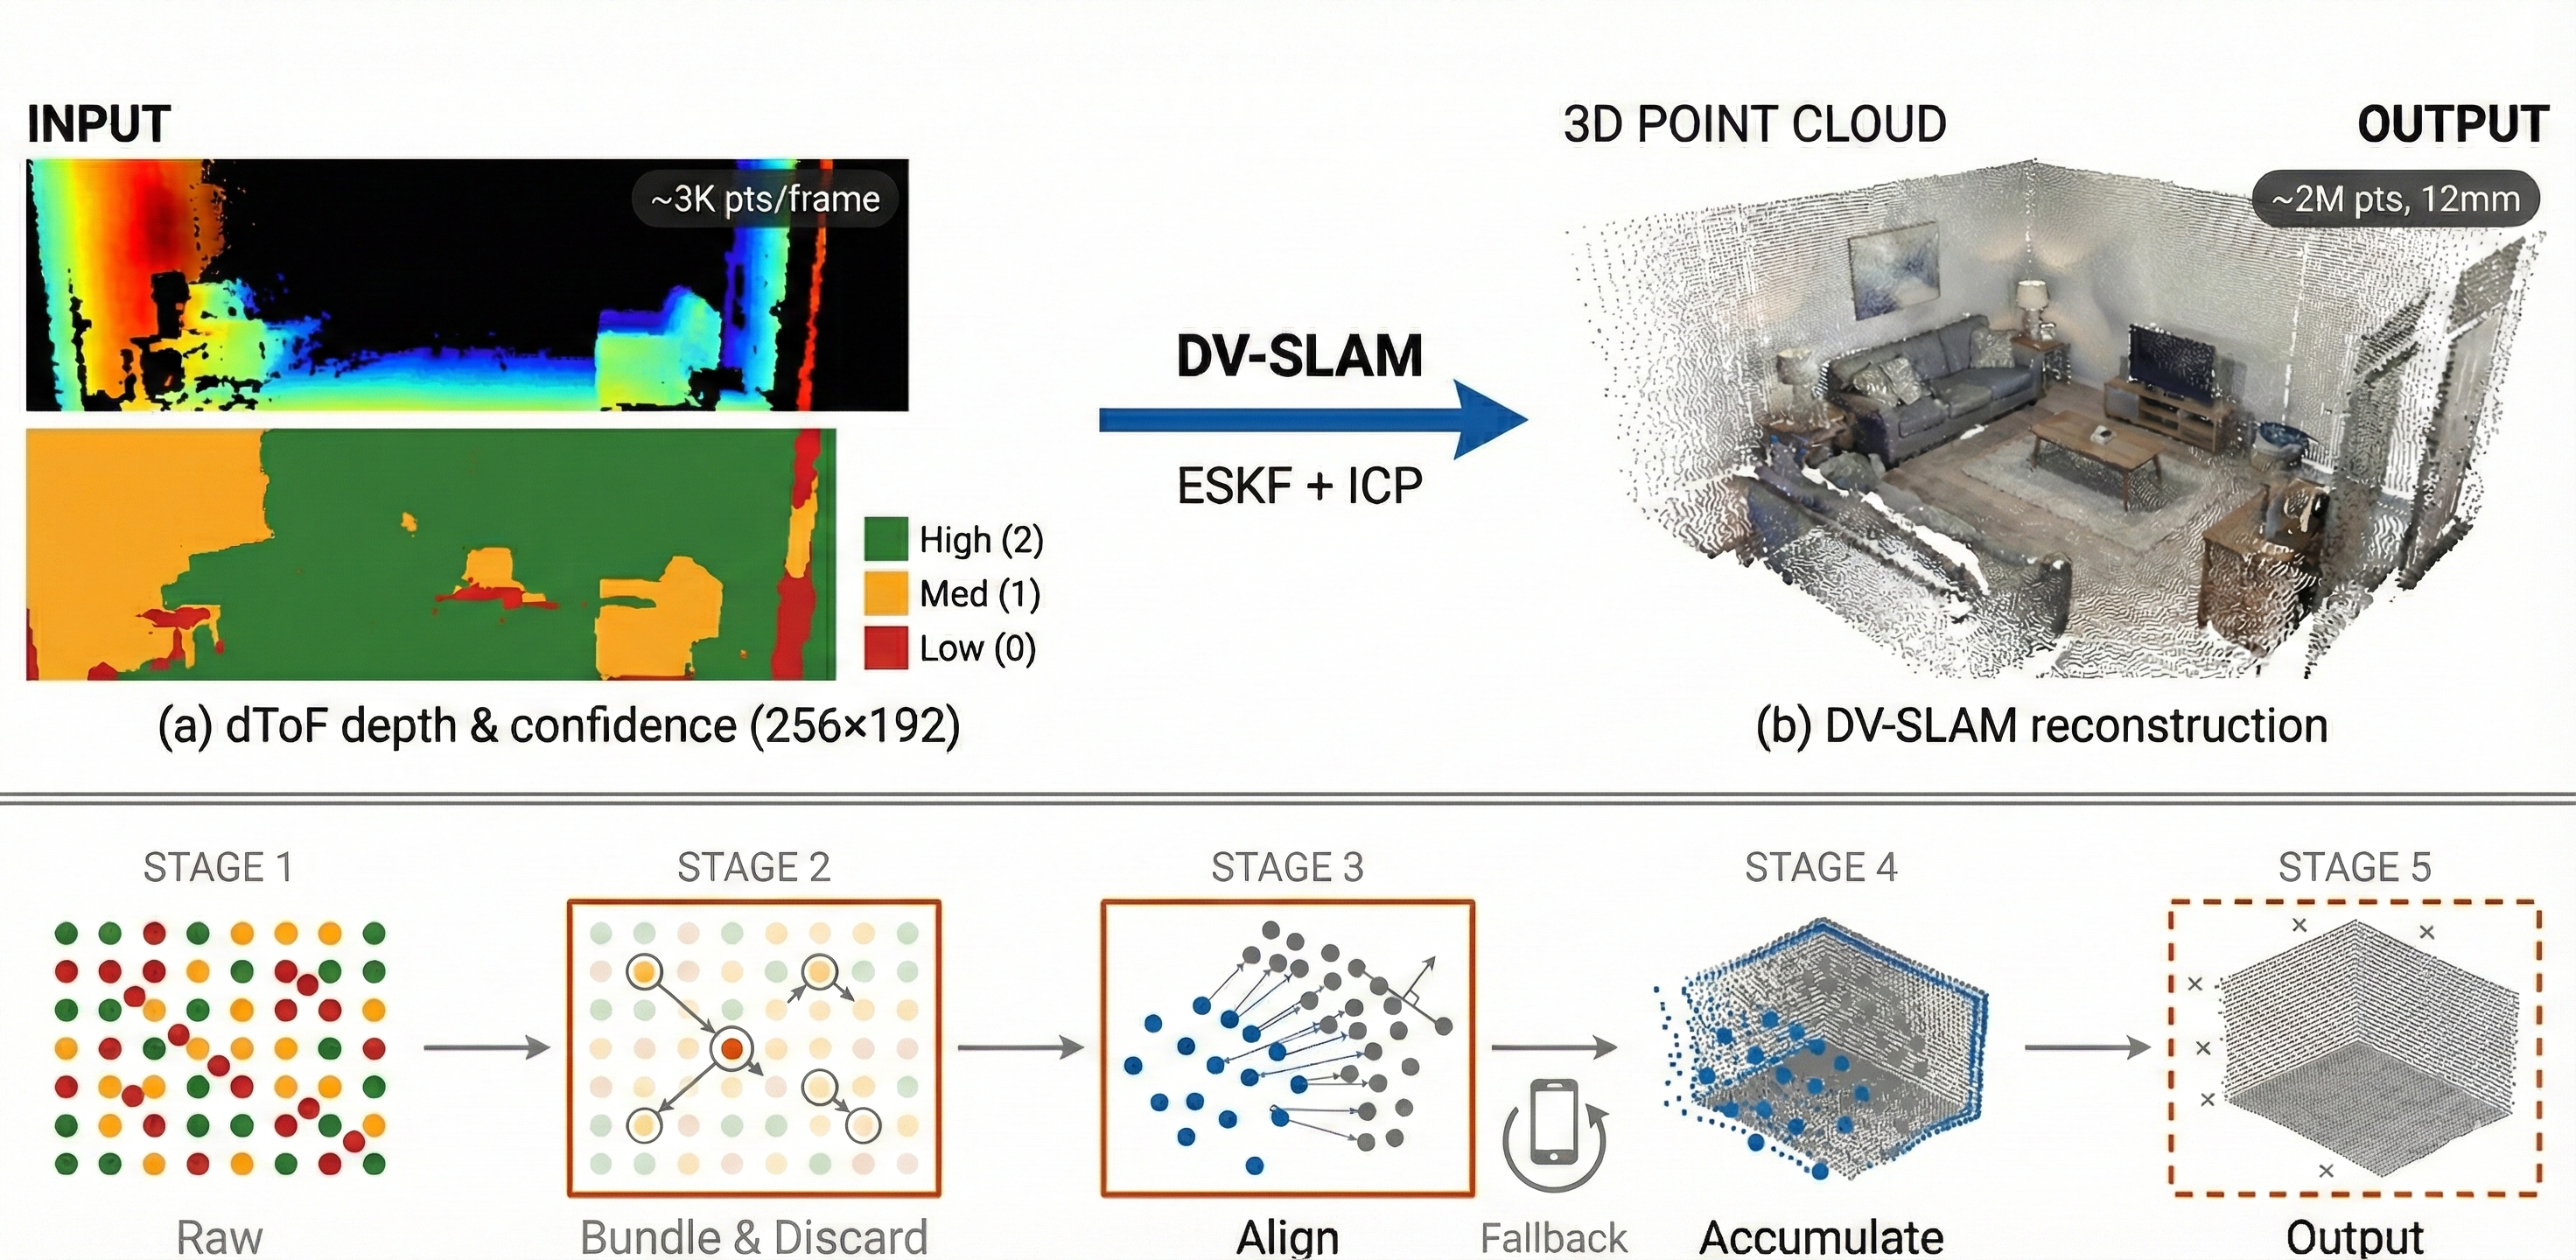
\includegraphics[width=\textwidth]{dvslam_fig1.png}
    \caption{Overview of DV-SLAM.
    (a)~Input: a single dToF frame produces a $256\!\times\!192$ depth map
    (${\sim}$3K pixels; ${\sim}$200--500 usable points after filtering)
    alongside a monocular camera image and 100\,Hz IMU data.
    (b)~Output: accumulated 3D point cloud at ${\sim}$12\,mm spacing.
    Bottom: the five-stage pipeline running at 30\,Hz on-device.}
    \label{fig:overview}
\end{figure*}

Since 2020, hundreds of millions of smartphones have shipped with
direct time-of-flight (dToF) LiDAR sensors operating on the same
single-photon avalanche diode (SPAD) principle as research-grade
flash LiDARs~\cite{luetzenburg2021evaluation}.
The dToF module on recent devices produces $256 \times 192$ depth maps
at 30\,Hz (Table~\ref{tab:sensor_comparison}).
After conservative quality filtering, only 200--500 points survive per
frame — two orders of magnitude fewer than a typical
mechanical LiDAR scan.
Quantization noise (1--5\,cm), multipath on reflective surfaces,
and range-dependent degradation make dToF point quality highly
non-uniform, unlike mechanical LiDARs where uniformity can be assumed.

\begin{table}[t]
    \centering
    \caption{Sensor comparison: consumer dToF vs.\ mechanical scanning
    LiDARs commonly used in LIO benchmarks.
    Consumer dToF column shows specifications of the Apple dToF module;
    Android dToF sensors have comparable resolution and range.}
    \label{tab:sensor_comparison}
    \setlength{\tabcolsep}{3.5pt}
    \begin{tabular}{lccc}
        \toprule
        Specification    & Consumer dToF    & VLP-16           & OS1-64           \\
        \midrule
        Principle        & SPAD photon cnt. & ToF rotating     & ToF rotating     \\
        Resolution       & $256 \times 192$ & 16 ch.           & 64 ch.           \\
        Points / frame   & ${\sim}$200--500 & ${\sim}$30K      & ${\sim}$131K     \\
        Range accuracy   & 1--5\,cm         & $\pm$3\,cm       & $\pm$2.5\,cm     \\
        Max range        & ${\sim}$5\,m     & 100\,m           & 90\,m$^\dagger$  \\
        FOV (H$\times$V) & $60\times48^{\circ}$ & $360\times30^{\circ}$ & $360\times45^{\circ}$ \\
        Per-point quality & 3-level conf.   & None             & None             \\
        Cost             & Consumer phone   & ${\sim}$\$4K$^\ddagger$ & ${\sim}$\$6K+ \\
        \bottomrule
        \multicolumn{4}{l}{\scriptsize $^\dagger$At 10\% reflectivity.
                           $^\ddagger$Discontinued (Ouster acquisition).}
    \end{tabular}
\end{table}

%% P3: The sparse regime is qualitatively different — three failure modes
This is not a scaled-down version of dense LIO; the sparse dToF regime
is \emph{qualitatively different}.
Dense-cloud systems (FAST-LIO2, DLIO, LIO-SAM~\cite{shan2020liosam})
do not gracefully degrade to $<$500-point data,
because three failure modes absent in the dense regime become dominant:

\begin{itemize}
    \item[\textbf{F1.}] \textbf{ICP rank deficiency.}
    With $<$500 points spanning a narrow field of view ($60\times45^{\circ}$),
    the observation matrix frequently lacks sufficient geometric diversity
    for a well-conditioned 6-DoF update.
    Dense LIO with 10K+ points rarely encounters this.

    \item[\textbf{F2.}] \textbf{Single-point dominance.}
    When only 200--500 points contribute to the Kalman update,
    a single erroneous correspondence can corrupt the entire pose estimate.
    In dense LIO, one bad point among 10K is noise.

    \item[\textbf{F3.}] \textbf{Blind downsampling destruction.}
    Standard voxel downsampling applied to 500 points can reduce them
    to $<$50, obliterating geometric constraint.
    Dense LIO can downsample 10K$\rightarrow$1K and still function.
\end{itemize}

%% P4: Existing mobile systems do not solve this
The only widely deployed solutions on consumer dToF devices are
the manufacturer's closed-source visual-inertial odometry (VIO) and
open-source wrappers (e.g., RTAB-Map~\cite{labbe2019rtabmap}) that
delegate their front-end entirely to this platform VIO.
Both treat the dToF sensor as a passive depth source and offer no
on-device LIO capability.
Recent work attaching an external Livox Mid-360 to an Android
smartphone~\cite{liu2025livoxphone} addresses mobile computation
but not sensor sparsity: the external sensor delivers ${\sim}$200K
points/scan and a full $360^{\circ}$ field of view, bypassing the
sparse-regime problem entirely.
To our knowledge, no peer-reviewed LIO system has been designed
for, or systematically evaluated on, the sub-500-point regime
inherent to built-in mobile dToF sensors.

%% P5: Our answer — lightweight LIO architecture for sparse dToF
We ask: \emph{can tightly-coupled LIO operate robustly below 500 points
per frame using only the sensors built into a modern smartphone,
and if so, what architectural principles are required?}

We answer affirmatively with DV-SLAM (Fig.~\ref{fig:overview}),
a LiDAR-inertial-visual odometry system designed from the ground up
for sparse mobile dToF hardware.
The pipeline fuses depth point-to-plane residuals, monocular visual
reprojection residuals, and IMU propagation in a single iterated ESKF
update, running at 30\,Hz on-device on an iPhone\,15\,Pro\,Max
with no GPU offloading and no external hardware.
Unlike prior mobile mapping systems, all processing — IMU propagation,
visual feature tracking, and point-to-plane ICP — runs entirely on
the smartphone's own compute with a single Eigen dependency.

%% P6: Contributions (3 only — clean)
In summary, our contributions are:

\begin{enumerate}
    \item \textbf{First on-device LIO for sparse mobile dToF.}
    We demonstrate tightly-coupled LiDAR-inertial-visual odometry
    operating at 30\,Hz on a smartphone using only its built-in dToF,
    camera, and IMU — without ARKit VIO poses, external LiDAR, or
    offloading computation.
    This is, to our knowledge, the first LIO system validated on the
    sub-500-point regime inherent to built-in mobile dToF sensors.

    \item \textbf{Sparse-regime characterization.}
    A point-count sweep (50--3{,}000 points/frame) provides the first
    empirical characterization of the LIO collapse boundary in the
    sparse dToF regime, quantifying how trajectory error degrades as
    the per-frame observation count decreases toward the minimum viable
    threshold for stable odometry.

    \item \textbf{Lightweight mobile LIO architecture.}
    We replace the ikd-tree used by FAST-LIO2 with an O(1)-insert
    voxel hash map with LRU eviction (500K-cell cap), cap ESKF updates
    at 100 stride-sampled observations per frame (125$\times$ LDLT
    reduction), and eliminate all PCL/ROS/Boost/Sophus dependencies
    in favor of Eigen-only self-contained code with fixed-size
    stack arrays (\texttt{VoxelCell[20]}, \texttt{KNN[5]},
    ring-buffer IMU queue).
    The result is a ${\sim}$3\,MB binary that runs at 30\,Hz on an
    Apple A17 Pro SoC.
\end{enumerate}

Source code will be released upon acceptance.
